%In this section we propose a regularized version of the Kantorovich-Rubinstein problem and we prove that it is still the dual of a transportation problem. Furthermore, we show that it has good properties in terms of robustness for classification problem.
\subsection{Definitions and primal transportation problem}
%\begin{figure}
%  \centering
%  \includegraphics[width=0.7\linewidth]{img/loss_function.png}
%  \caption{$\mathcal{L}_{\W pen}$ loss function with respect to $yf(x)$.}
%  \label{fig:loss}
%\end{figure}%
In order to improve the classification abilities of the classifier based on Wasserstein distance, we propose a Kantorovich-Rubinstein optimization problem regularized by an hinge loss :


\begin{equation} \label{eq:reg_OT} 
\begin{split} 
\sup_{f \in Lip_1(\Omega)}&-\mathcal{L}^{hKR}_\lambda(f) =\\ & \inf_{f \in Lip_1(\Omega)} \underset{\textbf{x} \sim P_-}{\mathbb{E}} \left[f(\textbf{x})\right]-\underset{\textbf{x} \sim P_+}{\mathbb{E}}\left[f(\textbf{x})\right] \\ &+\lambda\underset{\textbf{x}}{\mathbb{E}} \left(1-Yf(\textbf{x})\right)_+ \end{split} 
\end{equation}

where $(1-\textbf{y}f(\textbf{x}))_+$ stands for the hinge loss $max(0,1-\textbf{y}f(\textbf{x}))$ and $\lambda>=0$. We name $\mathcal{L}^{hKR}_\lambda$ the hinge-KR loss. The goal is then to minimize this loss with an 1-Lipschitz neural network.
When $\lambda=0$, this corresponds to the Kantorovich-Rubinstein dual optimization problem. Intuitively, the 1-Lipschitz function $f^*$ optimal with respect to Eq.~\eqref{eq:reg_OT} is the one that both separates the examples with a margin and spreads as much as possible the image of the distributions. When using only an hinge loss (as in \cite{li2019preventing} for instance), the examples outside the margin are no more taken into consideration. If the margin is increased to cover all the examples and if the class are equally distributed, the hinge loss becomes equivalent to the Kantorovich Rubinstein loss and then leads to a weak classifier. 

In the following, we introduce Theorems that prove the existence of such an optimal function $f^*$ and important properties of this function. Demonstrations of these theorems are in Appendix~\ref{appendix:proofs}.
\begin{Theorem} [Solution existence]
\label{Lemma:bounded_M}
 For each $\lambda>0$ there exists at least a solution $f^*$ to the problem  \[ f^*:=f_{\lambda}^*\in{\arg\min}_{f\in \text{Lip}_1(\Omega)}\mathcal{L}^{hKR}_{\lambda}(f) . \]
\end{Theorem}
Moreover, let $\psi$ be an optimal transport potential for the transport problem from $P_+$ to $ P_-$, $f^*$ satisfies that 
\begin{align}\label{eq:M}
	|| f^*||_{\infty}\leq M:= 1+\text{diam}(\Omega)+\frac{L_1(\psi)}{\inf(p,1-p)}.
\end{align}
%\footnote {{\color{red} (Franck) ne faudrait-il pas commenter l'apport de cette inégalité?  ?}}
The next theorem establishes that the Kantorovich-Rubinstein optimization problem with hinge regularization is still a transportation problem with relaxed constraints on the joint measure (which is no longer a joint probability measure).
\begin{Theorem}[Duality]\label{Theo:dual}
Set  $P_+, P_-\in \mathcal{P}(\Omega)$ and $\lambda>0$, then the following equality holds
\begin{align}\label{eq:dual}
\begin{split}
 \sup_{f\in \text{Lip}_1(\Omega)}- \mathcal{L}^{hKR}_\lambda(f)=&	\inf_{\pi \in\Pi^p_{\lambda}(P_+, P_-)}\int_{\Omega\times \Omega}|{\textbf{x}}-{{\textbf{z}}} |d\pi\\
 & + \pi_{\textbf{x}}(\Omega)+\pi_{{\textbf{z}}}(\Omega)-1
	\end{split}
\end{align}
Where $\Pi^p_{\lambda}(P_+, P_-)$ is the set consisting of positive measures $\pi\in \mathcal{M}_+(\Omega\times \Omega)$ which  are absolutely continuous with respect to the joint measure $dP_+\times dP_-$ and $\frac{d\pi_{\textbf{x}}}{dP_+}\in [p, p(1+\lambda)]$, $\frac{d\pi_{{\textbf{z}}}}{dP_-}\in [1-p, (1-p)(1+\lambda)] $.
%\footnote {{\color{red} (Franck) $[p, p(1+\lambda)]$ et $[1-p, (1-p)(1+\lambda)]$ me paraitrait plus clair}}
\end{Theorem}
%When the class are balanced, the constraints on $\pi$ became $\frac{d\pi_{\textbf{x}}}{d\mu}\in [\frac{1}{2}, \frac{1}{2}+\frac{1}{2}\lambda]$, $\frac{d\pi_{{\textbf{z}}}}{d\nu}\in [\frac{1}{2}, \frac{1}{2}+\frac{1}{2}\lambda] $ \footnote {{\color{red} (Franck) utile? obvious}}


\subsection{Classification and geometrical properties}
\label{sec:khr_properties}

\begin{figure*}
\centering
\begin{subfigure}{.4\textwidth}
  \centering
  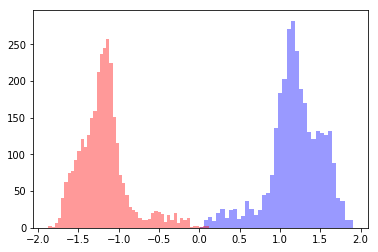
\includegraphics[width=0.8\linewidth]{img/wass_reg_2moons_dist.png}
  \caption{Distribution of $\hat{f}$ conditionally to the classes.}
  \label{wass_pen:sub1}
\end{subfigure}%
\begin{subfigure}{.36\textwidth}
  \centering
  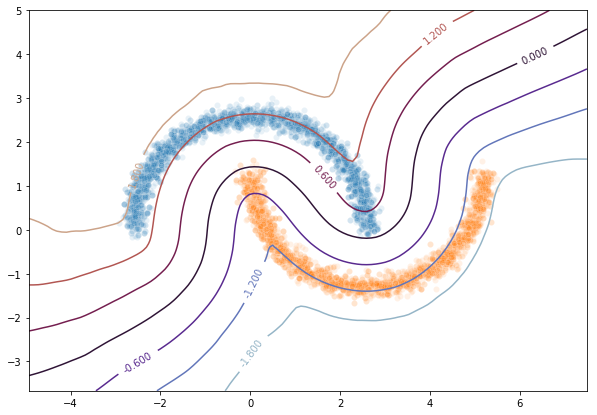
\includegraphics[width=1\linewidth]{img/wass_reg_2moons_class.png}
  \caption{Level map of $\hat{f}$}
  \label{wass_pen:sub2}
\end{subfigure}
\caption{Hinge regularized Kantorovich-Rubinstein (hinge-KR) classification on the two moons problem}
\label{fig:wass_pen}
\end{figure*}
We note $\hat{f}$ the solution obtained by minimizing $\mathcal{L}^{hKR}_\lambda$ on a set of labeled examples and $f^*$ the solution of Eq.~\eqref{eq:reg_OT}. We don't assume that the solution found is optimal (i.e. $\hat{f}\neq f^*$) but we assume that $\hat{f}$ is 1-Lipschitz. Given a function $f$, a classifier based on $sign(f)$ and an example $x$, an adversarial example is defined as follows:
\begin{equation}
    adv(f,\textbf{x})=\underset{\textbf{z}\in \Omega | sign(f(\textbf{z}))=-sign(f(\textbf{x}))}{argmin}\parallel \textbf{x}-\textbf{z}\parallel.
\end{equation}
According to the 1-Lipschitz property of $\hat{f}$ we have 
\begin{equation}
\label{lowerbound}
%\parallel x- adv(\hat{f},x) \parallel \geq |\hat{f}(x)|.
|\hat{f}(\textbf{x})| \leq |\hat{f}(\textbf{x})-\hat{f}(adv(\hat{f},\textbf{x}))| \leq \parallel \textbf{x}- adv(\hat{f},\textbf{x}) \parallel.
\end{equation}
So $|\hat{f}(\textbf{x})|$ is a lower bound of the distance of $x$ to the separating boundary defined by $\hat{f}$ and thus a lower bound to the robustness to $l_2$ adversarial attacks. Thus, by minimizing $\mathbb{E} \left((1-\textbf{y}f(\textbf{x}))_+\right)$, we maximize the accuracy of the classifier and by maximizing the discrepancy of the image of $P_+$ and $P_-$ with respect to $f$ we maximize the robustness with respect to adversarial attack. The proposition below establishes that the gradient of the optimal function with respect to Eq.~\eqref{eq:reg_OT} has norm 1 almost surely, as for the unregularized case (Eq.~\eqref{eq:nabla_1}).
\begin{Proposition}\label{coro_norm1}
Let $\pi$ be the optimal measure of the dual version \eqref{eq:dual} of the hinge regularized optimal transport problem. Suppose that it is absolutely continuous with respect to Lebesgue measure. Then there exists at least a solution $f^*$ of \eqref{eq:dual} such that $||\nabla f^*||=1$ almost surely.
\end{Proposition}
 %Even we haven't prove it formally yet, empirical results suggest that given $\textbf{x}$, the image $tr_{f^*}(\textbf{x})$ of $\textbf{x}$ with respect to the transportation plan and $adv(\textbf{x})$ are in the same direction with respect to $x$ and this direction is $-f^*(\textbf{x})*\nabla_x f^*(\textbf{x})$ (i.e $adv(\textbf{x})\approx x-c_x*f^*(\textbf{x})*\nabla_x f^*(\textbf{x})$ and $tr_{f^*}(\textbf{x})\approx x-c'_x*f^*(\textbf{x})*\nabla_x f^*(\textbf{x})$ with $0 \leq c_x \leq c_x' \in \mathbb{R} $). This would link the adversarial attack to the optimal transport.
Furthermore, empirical results suggest that given $\textbf{x}$, the image $tr_{f^*}(\textbf{x})$ of $\textbf{x}$ by transport plan and $adv(\textbf{x})$ are in the same direction with respect to $\textbf{x}$ and the direction is % and 
 $-\nabla_x f^*(\textbf{x})$. Combining this direction with the Eq.~\eqref{lowerbound}, we will show empirically (sect.~\ref{sec:experimentation}) that  $$adv(\textbf{x})\approx x-c_x*f^*(\textbf{x})*\nabla_x f^*(\textbf{x})$$ and $$tr_{f^*}(\textbf{x})\approx x-c'_x*f^*(\textbf{x})*\nabla_x f^*(\textbf{x})$$ with $1 \leq c_x \leq c_x' \in \mathbb{R} $. It turns out that this corresponds to the definition of FGSM attacks \cite{Goodfellow2014a}. This suggests that in our frameworks, adversarial attacks amount to travel along the transportation path from the example to its transportation image.
 
The next proposition shows that, if the classes are well separated, maximizing the hinge-KR loss leads to a perfect classifier.% with no error.
\begin{Proposition}[Separable classes]\label{coro:epsilon}
Set  $P_+, P_-\in \mathcal{P}(\Omega)$ such that $P(Y=+1)=P(Y=-1)$ and $\lambda\geq 0$ and suppose that there exists $\epsilon>0$ such that
\begin{align}\label{coro:hipotesis}
	| {\textbf{x}}-{\textbf{{{\textbf{z}}}}} |> 2 \epsilon \ \ dP_+\times dP_- \text{ almost surely}
\end{align}
Then for each
\begin{align*}
	f_{\lambda}\in {\arg\sup}_{f\in \text{Lip}_{1/\epsilon}(\Omega)}\int_{\Omega}f(dP_+-dP_-)-\\
	\lambda \left( \int_{\Omega}(1-f)_+dP_+ +\int_{\Omega}(1+f)_+dP_-\right),
\end{align*}
it is satisfied that $L_1(f_{\lambda})=0.$ Furthermore if $\epsilon\geq 1$ then $f_{\lambda}$ is an optimal transport potential from $P_+$ to $P_-$ for the cost $| {\textbf{x}}-{{\textbf{z}}}|$.
\end{Proposition}
We show in Fig.~\ref{fig:wass_pen}, on the two moons problem, that in contrast to the vanilla classifier based on Wasserstein (Eq.~\eqref{eq:wass_vanilla_classif}), the proposed approach enables non overlapping distributions of $\hat{f}$ conditionally to the classes (Fig.~\ref{wass_pen:sub1}).
%Figure~\ref{fig:wass_pen} illustrates the approach on the two moons problem. Contrarily to the example with Wasserstein, we observe that the distributions of $f$ conditionally to the classes doesn't overlap (Figure~\ref{wass_pen:sub1}). 
In the same way, the 0-level cut of $\hat{f}$ (Fig.~\ref{wass_pen:sub2}) is a nearly optimal classification boundary. Moreover, the level cut of $\hat{f}$, on the support of the distributions, is close to the distance to this classification boundary.
%, corresponds approximately to the distance to the classification boundary.  